\documentclass{ximera}
\title{Mean Value Theorem}
\begin{abstract}
\end{abstract}
\begin{document}
\maketitle
\subsubsection{Introduction}
\begin{dialogue}
\item[Dylan] I don't know about this theorem...it seems pretty \textit{mean}...
\item[Julia] No no, they mean \textit{mean} as in average!
\item[Dylan] Oh, so were looking at the average value of a function?
\item[James] Not quite, actually the \textbf{mean value theorem} states the following: If $f$ is continuous on $[a,b]$ and differentiable on $(a,b)$, then there exists at least one value $c$ in $(a,b)$ such that $$f'(c)=\frac{f(b)-f(a)}{b-a}$$
\item[Dylan and Julia] Maybe we should do an example...that looks pretty confusing...
\item[ALTOGETHER] Let's dive in!
\end{dialogue}
\subsubsection{Guided Example}
Take a look at the following graph illustrating the Mean Value Theorem
\begin{figure}
    \centering
    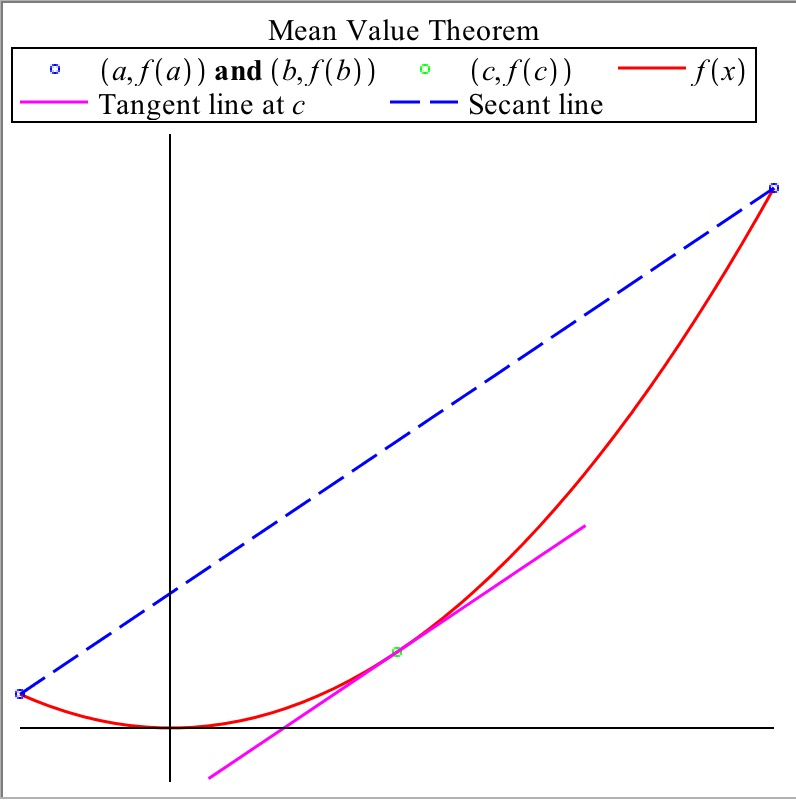
\includegraphics[width=80mm]{meanvalue.jpg}
    \label{fig:meanvalue}
\end{figure}
\begin{question}
What do you notice about the tangent line at c with respect to the secant line from a to b?
\begin{freeResponse}
\end{freeResponse}
What does this mean the derivative of $f(x)$ is at $c$?
$\answer{0}$
\end{question}
\begin{question}
If $f'(x)$ was zero for all points in the interval, what could be said about $f(x)$ on that interval?
$\answer{f'(x) is constant}$
\end{question}
\begin{question}
Use $f(x)=sin(2x)$ on the interval $[0,2\pi]$ for the following questions.

Graph $f(x)$
\[
\graph{}
\]

What values for $c$ satisfy the mean value theorem?

$\answer{\pi/4,3\pi/4,5\pi/4, 7\pi/4}$
\end{question}
\subsubsection{On Your Own}
\[
\graph{|x^2-x-2|}
\]
Let $f(x)=\left|x^2-x-2\right|$.
\begin{question}
Examine the graph, does the Mean Value Theorem apply to $f$ on the interval $[a,b]=[0,3]$?

$\answer{Yes}$
If the theorem does apply, for what value of $x$ is the theorem satisfied?

$\answer{}$
\end{question}
\begin{question}
\[
\graph{1/x}
\]
Consider $f(x) = \frac{1}{x}$.

Over what region does the Mean Value Theorem not apply?

\begin{freeResponse}
\end{freeResponse}

Apply the Mean Value Theorem from [1, 4], determining what points experience the same instantaneous change as the entire interval.
\begin{freeResponse}
\end{freeResponse}
\end{question}
\begin{question}
Seeing a police officer on the side of the road, your friend Tom slows down to 35 mph. However, once the officer pulls over someone else for speeding, Tom speeds up to 70 mph. Half an hour and 35 miles later, Tom checks his navigation app and sees another police officer is up ahead, slowing himself down to the legal 35 mph. However, the police officer still pulls Tom over, saying he had been radioed by the first officer right when Tom passed, so he could prove that Tom was going 70 mph at some point in the last half hour. Tom is furious about the clearly faulty reasoning of the police officer.

Thanks to the Mean Value Theorem, you know the police officer is in the right. Using $g(x)$ as a function of position to time, explain to Tom why the officer had a valid reason to ticket him.

\begin{freeResponse}
\end{freeResponse}

Talking to Tom, you find out that he accelerated to 70 mph in only 5 seconds after passing the officer. Prove that at some point, Tom had an acceleration of over 25,000 $\frac{\text{mi}}{\text{h}^2}$.

\begin{freeResponse}
\end{freeResponse}
\end{question}

\subsubsection{In Summary}
\begin{definition}
The \textbf{Mean Value Theorem} states that for any function $f$, if $f$ is continuous on $[a,b]$ and differentiable on $(a,b)$, then there exists at least one value $c$ such that $$f'(c)=\frac{f(b)-f(a)}{b-a}$$

This means that there is a point $c$ such that the secant line from $a, b$ has the same slope as the tangent line at $c$. It's important to note that this means if $f'(x)=0$ for all $x$ on $(a,b)$, then $f$ is constant on $(a,b)$.
\end{definition}
\end{document}